\documentclass[conference]{IEEEtran}

\usepackage{graphicx}

\graphicspath{ {images/} }


\usepackage{listings}
\usepackage{color}

\definecolor{dkgreen}{rgb}{0,0.6,0}
\definecolor{gray}{rgb}{0.5,0.5,0.5}
\definecolor{mauve}{rgb}{0.58,0,0.82}

\lstset{
	language=Java,
	aboveskip=3mm,
	belowskip=3mm,
	showstringspaces=false,
	columns=flexible,
	basicstyle={\small\ttfamily},
	numbers=none,
	numberstyle=\tiny\color{gray},
	keywordstyle=\color{blue},
	commentstyle=\color{dkgreen},
	stringstyle=\color{mauve},
	breaklines=true,
	breakatwhitespace=true,
	tabsize=3
}





\begin{document}
	\title{Hadoop Image Processing Framework}
	\author{\IEEEauthorblockN{Sridhar Vemula}
		\IEEEauthorblockA{Computer Science Department\\
			Oklahoma State University\\
			Stillwater, Oklahoma \\
			Email: sridhar.vemula@okstate.edu}
		\and
		\IEEEauthorblockN{Christopher Crick}
		\IEEEauthorblockA{Computer Science Department\\
			Oklahoma State University\\
			Stillwater, Oklahoma \\
			Email: chriscrick@cs.okstate.edu}
	}
	\maketitle
	\begin{abstract}
		With the rapid growth of social media, the number of images being uploaded to the internet is exploding. Massive quantities of images are shared through multi-platform services such as Snapchat, Instagram, Facebook and WhatsApp; recent studies estimate that over 1.8 billion photos are uploaded every day.  However, for the most part, applications that make use of this vast data have yet to emerge. Most current image processing applications, designed for small-scale, local computation, do not scale well to web-sized problems with their large requirements for computational resources and storage.  The emergence of processing frameworks such as the Hadoop MapReduce\cite{Hadoop2009} platform addresses the problem of providing a system for computationally intensive data processing and distributed storage. However, to learn the technical complexities of developing useful applications using Hadoop requires a large investment of time and experience on the part of the developer.  As such, the pool of
		researchers and programmers with the varied skills to develop applications that can use large sets of images has been limited. To address this we have developed the Hadoop Image Processing Framework, which provides a Hadoop-based library to support large-scale image processing. The main aim of the framework is to allow developers of image processing applications to leverage the Hadoop MapReduce framework without having to master its technical details and introduce an additional source of complexity and error into their programs.
	\end{abstract}
	
	\IEEEpeerreviewmaketitle
	
	\section{Introduction}
	With the spread of social media in recent years a large amount of image data is accumulated. Processing this large image data is limited to single computer which lack in computational power and storage ability. These tasks typically be performed on a distributed system by dividing the task into sever sub tasks. The ability to parallelize tasks allows for scalable, efficient, execution of resource-intensive applications. Hadoop MapReduce framework provides a platform for such tasks.
	
	Also, when considering operations such as face detection, image classification\cite{Li2009} and other types of processing on images, there are limits on what can be done to improve performance of single computers to make them able to process large-scale information. Therefore, the advantages of parallel distributed processing of a large image dataset by using the computational resources of cloud computing environment can be considered. In addition, if computational resources can be secured easily and relatively inexpensively, then cloud computing in suitable for handling large size image data sets at very low cost and increased performance. Hadoop, as a system for processing large numbers of images by parallel and distributed computing seems promising. In fact, Hadoop is in use all over the world. Studies using Hadoop have been performed to treat one file as a text data file or multiple files as a single file unit, such as for the analysis of large volumes of DNA sequence data, converting the data of a large number of still images to PDF format, and carrying out feature selection/extraction in astronomy. These examples demonstrate the usefulness of this system, which is due to its having the ability to run multiple processes in parallel for load balancing and task management.
	
	Most of the image processing applications, that use Hadoop MapReduce framework require a staggering learning curve and high complexity. The overhead required to implement such applications is cumbersome to users. Hadoop Image Processing Framework hides the highly technical deatails of Hadoop system and provides users with a feel of an normal image processing library giving the users the access to advanced resources of distributed system. Our framework mainly focuses around giving users an easy way to access the image data allowing for easy and flexible use for large scale image applications
	
	Hadoop Image Processing Framework is largely a software design project, with a goal of hiding Hadoop's functionality and provide users with a library to effectively use Hadoops MapReduce system for large scale image processing. We believe that the ease of use and java oriented semantics will make the process of creating large scale image experiments further more easier. This framework is an excellent tool for Hadoop novice users and image processing researchers because it allows development of large scale image processing applications.
	
	In the following section  we will describe prior work in this area. Next we describe the overview for the Hadoop Image Processing Framework including the Downloader, Processor and Extractor statges. Additionally, we describe our approach of distributing tasks for MapReduce. Finally we demonstrate the potential of this framework with a few examples of image processing.
	
	\section{Prior Work}
	With rapid increase of usage of online photo storage and social media like facebook, flickr and picasa the amount of image data available is larger than ever before. The amount of image data is growing rapidly every day. According to Buzzfeed for every minute 27800 photos are uploaded to Instagram. As per facebook, they get 208,300 photos uploaded every minute\cite{Horaczek2013}. This alone provides a plethora of image that can scale up to billions of images. It is these reasons that motivate the need for research with image processing applications that take advantage of large sets of images
	
	A brief overview of previous work sharing the themes of image processing and distributed computation is presented below:
	
	Web-Scale Computer Vision using MapReduce for Multimedia Data Mining \cite{White2010} present a case study of classifying and clustering billions of regular images using MapReduce. A way of pre-processing images for use in a sliding-window approach for object recognition is described. Distributed High Performance Video Processing in the cloud, outlines some of the limitations of the MapReduce model when dealing with high-speed video encoding, namely its dependence on the NameNode as a single point of failure, and lack of possibility for generalization in order to suit the issue at hand. An alternate optimized implementation is proposed for providing cloud-based IaaS (Infrastructure as a Service) Solution. In Parallel K-Means clustering of Remote Sensing Images Based on MapReduce \cite{Lv2010} describe using the k-means algorithm in conjunction with MapReduce and satellite/aerophoto images in order to find different elements based on their color. Using Transaction Based Parallel computing to solve image processing and computational physics problems by Harold describes the use of distributed computing with two examples video processing and subsurface transport. There was no information provided on how image processing parts of the examples. 
	
	Case Study of Scientific Data Processing on a Cloud Using Hadoop \cite{Zhang2010} present methods used for processing sequences of microscope images of live cells. The images are relatively small 512x512 16-bit pixels, stored in 90 MB folders there were some issues regarding to fitting into Hadoop DFS blocks with were solved by custom InputFormat, InputSplit and Record Reader classes. A scalable image processing framework for gigapixel Mars and other celestial body images by Mark Powell describes the way NASA handles image processing of celestial images captured by the Mars Orbiter and rovers. Clear and concise descriptions are provided about the segmentation of gigapixel images into tiles, how the tiles are processed and how image processing framework handles scaling and works with the distributed processing. Ultra-fast processing of gigapixel tissue microarray images using high performance computing \cite{Wang2011} about the speeding up the analysis of Tissue MicroArray images by substituting human expert analysis for automated processing algorithms. While the images were measured to be in gigapixels, the content is easily segmented and there was no need to focus on being able to analyze all of image at once. The work was all done on a specially build grip high performance	computing platform on Hadoop framework. 
	
	Terabyte size image computations on Hadoop cluster \cite{Bajcsy2013} platforms present a characterization of four basic terabyte size image computations on a Hadoop Cluster in terms of their relative efficiency according to the modified Amdahls law. The work is motivated by the fact that there is a lack of 6 standard benchmarks and stress tests for big image processing operations on Hadoop framework. Terabyte-scale image search\cite{Moise2013} outlines about querying thousands of images in one run using Hadoop MapReduce framework using the MapReduced based eCP Algorithm. The experiment does an image search on 110 million images collected from web on Grid 5000 Platform. The results are evaluated in order to understand the best practices that can tune Hadoop MapReduce Performance for image search.	
	
	While the above shows that there has been lot of work in this area, providing a framework to ease the process develop large-scale image processing applications. The question remains how the performance for Hadoop can be increased for large scale image processing tasks on small files.
	
\section{Methodology}
Hadoop Image processing Framework is created to provide users a tool to develop a large scale image processing applications with ease.

The main goals of Hadoop Image Processing framework:
\begin{itemize}
	\item Provide an open source framework over Hadoop MapReduce for developing large scale image applications 
	\item Flexibility to store images in various Hadoop File Formats
	\item Present users with an intuitive interface for image based operations which are highly parallelized and balanced and hide the high technical details of hadoop MapReduce Framework
	\item Allow interoperability between various image processing libraries
\end{itemize}

\subsection{Downloading and storing image data}
Hadoop's distributed file system(HDFS) to store files in various nodes throughout the cluster. Storing small files\cite{White2009} is a big problem in Hadoop. A small file is one which is significantly smaller than HDFS block size. As the large image dataset can have many number of small files and the problem is HDFS cant handle lots of files. The problem can be solved by providing some kind of container to group the files in some way. Hadoop offers a few options:
\begin{itemize}
	\item HAR File
	\item Sequence File
	\item Map File
\end{itemize}

The Downloader Module of the framework does the following work

\textbf{Step 1: Input a URL List.} Initially user inputs a file containing url's of images to download. The input list should be a text file with one image url per line. The list can be generated by hand, database or a search. The framework provides a extendable ripper module to extract urls from flickr, google and databases. In addition to the list the user will input the type of image bundle to be generated(e.g. har, sequence or map). According to the input, the urls are divided across the nodes for maximum efficiency and parallelism to download the images. Each node map task will generate few image bundles as per the input type containing all the of the images it downloaded. In the reduce phase, the Reducer will merge these image bundles  into a large image bundle.

\textbf{Step 2: Split URLs across nodes.}
From the input, file containing list of image urls and the type of file to be generated, we equally distribute the task of downloading images across the all the nodes in the cluster. The nodes are efficiently managed so that no memory overflow can occur even for terabytes of image downloaded by a single map task. This allows maximum parallelization for downloading. Image urls are distributed to all nodes equally and different map tasks begin downloading the image set it is responsible for.

\begin{figure}[h]
	\centering
	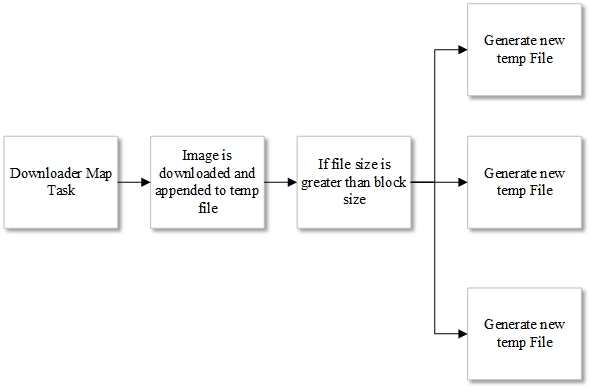
\includegraphics[width=0.45\textwidth]{down-map}
	\caption{Individual Map task of Downloader Module}
	\label{fig:down-map}
\end{figure}

\textbf{Step 3: Download image data from URLs.}
For every url retrieved in the map task, a connection is established as per transfer protocal (e.g. ftp, http, https etc.). Once connected, we check the file type and if its a valid image we get an InputStream to the connection. From this InputStream, we generate a new HImage object and add the image to the image bundle. The HImage class holds the image data and helps user to play with image and image header data. HImage class also provides an interoperability between various image data types (e.g. BufferedImage, Mat etc.,).

\textbf{ Step 4: Store images in an image bundle. } 
Once HImage object is received, we can add the image to the image bundle simply by passing the HImage object to the appendImage method. Each map task generates a few or many image bundles depending on the image list. In the reduce phase, all these image bundles are merged into one large bundle.

\begin{figure}[h]
	\centering
	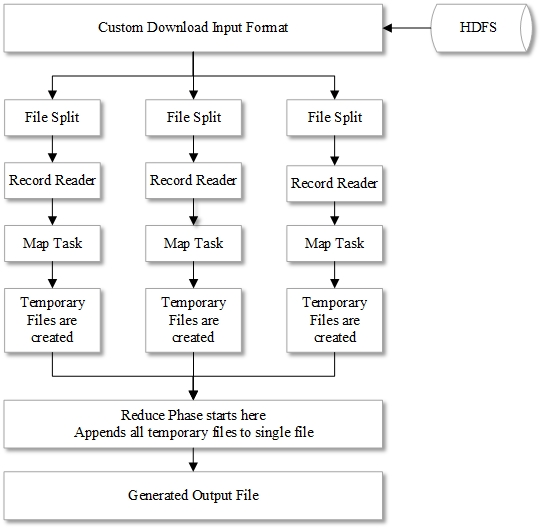
\includegraphics[width=0.45\textwidth]{down-node}
	\caption{Single Node running the Downloader Module handled by the framework and transparent to user}
	\label{fig:down-node}
\end{figure}



\subsection{Processing image bundle using MapReduce}
Hadoop MapReduce programs handle input and output data very efficiently, but the main problem is representing the image data. For instance, to distribute images across map nodes would require to pass images as string, then decode image into a specified format to access pixel information which is not only inefficient but also inconvenient. To overcome this problem we want to able to represent the images as many different formats to increase flexibility. The framework focuses on bringing familiar data types directly to user.

As distribution is important in MapReduce, we want to process the image in the same machine where the bundle block resides. In general, the user needs to create an InputFormat and Record Reader classes to specify the MapReduce job and distribute the input among nodes. This task is a bit cumbersome. In order to make the framework more easier we took care of the InputFormat and RecordReaders.

Images are distributed as various image data types and users can immediately have access to pixel values. As we attempt to obtain the pixel values we lose the valuable image header data(e.g. jpeg exif data, IHDR\cite{David03} Image Header). The framework, holds the image data in a special HImageHeader data type before converting the image bytes into pixel values. After working on the pixel data, it was made sure that image header is appended to the processed pixels. Even though it adds an storage overhead, image header data is preserved even after processing.

The working of Processor module of the framework is described below:

\textbf{Step 1: Input the Algorithm.} We assume that the user writes an algorithm which extends a Generic Algorithm class. This class is passed as an argument to the processor module. The framework starts a MapReduce Job with the algorithm as an input. The GenericAlgorithm holds an HImage variable, this helps user to write an algorithm on the single image which iterates over the whole image bundle. In addition to the algorithm the user should input the image bundle file that needs to be processed. According to the input the image bundle is divided across nodes as individual map task. Each Map task will process the image as of the algorithm and appends them to the output image bundle. In the reduce phase, the Reducer will merge these image bundles into a large image bundle.

\textbf{Step 2: Split Imagebundle across nodes.} The input image bundle is stored in HDFS as blocks. In order to obtain maximum throughput it was made sure the map task is run in the same the block where it resides, using custom input format and record reader classes. This allows maximum parallelization without a problem of transferring data across nodes. The image bundle now executes different map tasks for the image data it is responsible for.

\begin{figure}[h]
	\centering
	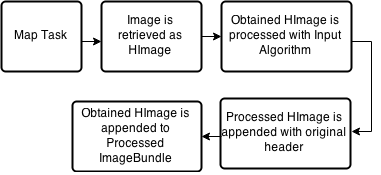
\includegraphics[width=0.45\textwidth]{pro-map}
	\caption{Individual Map task of Processor}
	\label{fig:pro-map}
\end{figure}

\textbf{Step 3: Process individual image.} For every HImage retrieved in the map task, the algorithm is run on the HImage which is given as the input to the processor module. The HImage retrieves the image as data type(e.g. BufferedImage, Mat image) in the algorithm. Once the image data type is retrieved processing takes place. After processing, the image header data of the original image is appended to the processed image, thereby preserving image header data. The processed image is appended to the temporary bundle generated by the map task.

\textbf{Step 4: Store processed images in an image Bundle.} Every map task generate a image bundle after the map task is completed. Once the map phase is completed there are many bundles. In the reduce phase, all these temporary image bundles are merged into a single large file which contains all the processed images.

\begin{figure}[h]
	\centering
	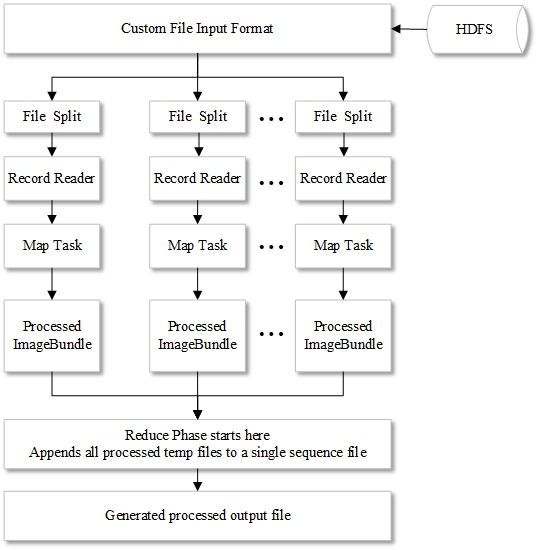
\includegraphics[width=0.45\textwidth]{pro-node}
	\caption{Single Node running the Processor Module handled by the framework and transparent to user}
	\label{fig:pro-node}
\end{figure}

\subsection{Extracting image bundle using MapReduce}
The framework creates and processes image bundles but there should be a way to extract these images and make them viewable. Generally, Hadoop extracts images from the image bundle iteratively using a single node which is not efficient. To make the process distributed among different nodes we designed an extractor module which can extract images in parallel in all the nodes. 

Distribution plays a key role in MapReduce, we want to make use of the nodes effectively to make the process of extraction efficient. In general, the user needs to create custom InputFormat and RecordReader classes to specify the MapReduce job and distribute the input among nodes. In order to over come this the framework takes care of these Custom InputFormat and RecordReader to make working with hadoop more easier.

There is often a confusion to where the images need to be extracted. The images can be extracted to the local file system of the node or hadoop file system. The framework overcomes the problem by providing a flexibility to choose.
 
The working of Extractor module is explained below.

\textbf{Step 1: Input the image bundle to be extracted.} The image bundle that needs to extracted is passed as a parameter to the Extractor module. Along with it the user can send an optional parameter to where the images need to be extracted (defaults to local file system). After the input the image bundle is distributed across nodes as individual map task. Each map task will extract the image in to the filesystem.     

\begin{figure}[h]
	\centering
	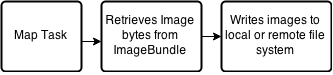
\includegraphics[width=0.45\textwidth]{ext-map}
	\caption{Individual Map Task of Extractor Module}
	\label{fig:ext-map}
\end{figure}


\textbf{Step 2: Split Image bundle across nodes}
The input image bundle split across nodes using the custom input format and record reader classes for maximum throughput. Once a Map task starts a HImage object is retrieved.

\textbf{Step 3: Extract individual image}
The obtained HImage object is retrieved as image bytes and the image bytes are stored into the file based on its image type. The Extractor module doesn't have a reduce phase.

\begin{figure}[h]
	\centering
	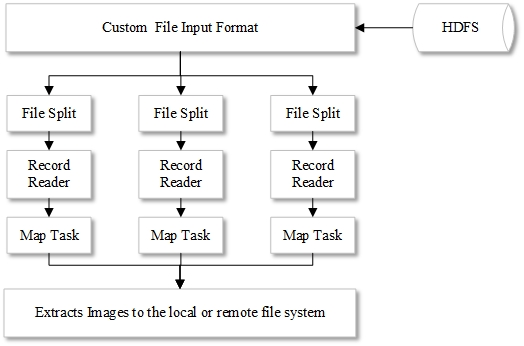
\includegraphics[width=0.45\textwidth]{ext-node}
	\caption{Single node running the Extractor Module handled by the framework and transparent to user}
	\label{fig:ext-node}
\end{figure}


\section{Experiments and Observations}

We describe two image applications using Hadoop Image Processing framework. These applications enable user perform large scale image processing operations with ease. These applications are complex and inefficient one existing platforms, yet simple to implement using the framework

\subsection{Canny Edge Detection}

Canny Edge Detection\cite{Canny86} is an multi-stage algorithm to detect a wide range of edges in images. Edge detection, especially step edge detection is an important technique to extract useful structural information from different vision objects and dramatically reduce the amount of data to be processed. Among the edge detection methods developed so far, canny edge detection algorithm is one of the most strictly defined methods that provides good and reliable detection.

\begin{figure}[h]
	\centering
	
\includegraphics[width=0.45\textwidth]{input-canny}
	\caption{A Sample Image from downloaded image bundle}
	\label{fig:input-canny}
\end{figure}

\begin{figure}[h]
	\centering
	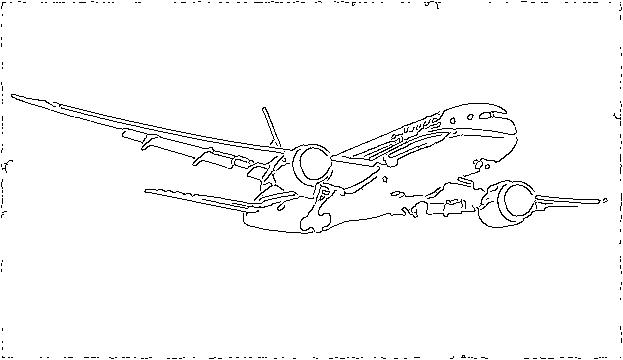
\includegraphics[width=0.45\textwidth]{output-canny}
	\caption{Processed image using canny edge detection}
	\label{fig:output-canny}
\end{figure}

\subsubsection{Characterstics of Image Dataset, Hardware and Software}
We computed edge detection on a dataset which is about 1TB size. The data set is made from the flickr search based on a keyword flight. The data set is extracted using the a FlickrRipper in the framework which implements Ripper Interface. The Ripper interface can be implemented for any custom Rippers to get the image URLs. The example data set is composed of 220000 images at 4.76 MB/image equals to 1 TB. We ran the edge detection on the cluster with 7 nodes having 2 to 4 virtual processors with 4 to 8 GB RAM. Each virtual processor clocks at a speed of 3.2 Ghz. The algorithm was implemented independently and used on single desktop, Hadoop cluster without framework and Hadoop cluster with framework.

\subsubsection{Observations}   

The desktop implementation of the Algorithm is a java program for processing a small image dataset. As soon as the data set is processed the program halts. The desktop implementation starts as a single thread. One image is processed every time. As soon as the image is processed, it starts processing a new image. When the data set size is low, the program runs smooth with best performance. As data set size increases to Terabytes the system can't handle such huge amounts of data. To handle such large amounts of data we use the distributed computing using hadoop.


\begin{figure}[h]
	\centering
	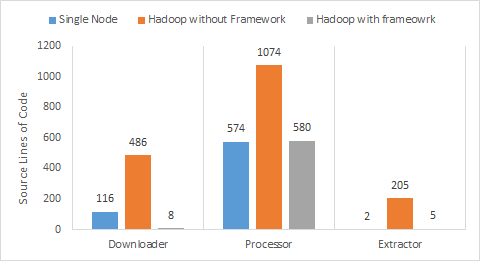
\includegraphics[width=0.45\textwidth]{module-chart}
	\caption{Module Chart}
	\label{fig:module-chart}
\end{figure}
 

The Algorithm is implemented on a hadoop cluster without using framework. It overcomes the problem of handling large datasets but suffers with a problem of code complexity. The user needs to write a huge amount of code and understand the technical details of hadoop. Writing such huge amounts of code including the custom InputFormats and RecordReaders is cumbersome. Fig.\ref{fig:module-chart} compares the actual lines of code user needs to write to run an Image Processing application in hadoop cluster which makes an average user life harder to use the hadoop features.

The Algorithm is finally implemented on a hadoop cluster using the framework. It overcomes many problems handling large datasets, code complexity, interoperability between image datatypes etc., The process of creating CustomInputFormat and RecordReader is automated as per the input. User can tune the settings using different getter and setter method to get the desired output. The framework is so transparent that the user needs to input few lines of code to process a large image data set. It hides all the MapReduce Technical details and runs the code highly parallelized. The key differences among the three platform-specific implementation lie in computation elasticity and code complexity associated with each platform.


\begin{table}[h]
	\begin{tabular}{|l|l|l|l|}
		\hline
		\multicolumn{1}{|c|}{\textbf{\begin{tabular}[c]{@{}c@{}}Computa-\\ tional\\ Platform\end{tabular}}} & \multicolumn{1}{c|}{\textbf{\begin{tabular}[c]{@{}c@{}}Computational \\ Elasticity\end{tabular}}}      & \multicolumn{1}{c|}{\textbf{\begin{tabular}[c]{@{}c@{}}Code \\ Complexity\end{tabular}}}                                                                                                                                                  & \multicolumn{1}{c|}{\textbf{\begin{tabular}[c]{@{}c@{}}Data \\ Locality\end{tabular}}}                                                                           \\ \hline
		Desktop                                                                                             & \begin{tabular}[c]{@{}l@{}}Low : limited by \\ RAM and CPU of \\ the executing\\ computer\end{tabular} & \begin{tabular}[c]{@{}l@{}}Normal : Complexity \\ lies in writing the \\ algorithm\end{tabular}                                                                                                                                           & \begin{tabular}[c]{@{}l@{}}All data are \\ on local disk\end{tabular}                                                                                            \\ \hline
		\begin{tabular}[c]{@{}l@{}}Hadoop:\\ without \\ using \\ framework\end{tabular}                     & \begin{tabular}[c]{@{}l@{}}High: Nodes can\\  be requested \\ as needed\end{tabular}                   & \begin{tabular}[c]{@{}l@{}}Heavy : Complexity \\ lies inwriting every \\ module in framework \\ including custom \\ Input Formats and \\ RecordReaders.User \\ should have high \\ technical knowledge on \\ hadoop working.\end{tabular} & \begin{tabular}[c]{@{}l@{}}All data resides\\ in HDFS. Custom\\ InputFormats \\ needsto be \\ created to launch\\ computations \\ where thedata are\end{tabular} \\ \hline
		\begin{tabular}[c]{@{}l@{}}Hadoop:\\ using \\ framework\end{tabular}                                & \begin{tabular}[c]{@{}l@{}}High: Nodes can \\ be requested \\ as needed\end{tabular}                   & \begin{tabular}[c]{@{}l@{}}Normal : Complexity \\ lies in writing \\ algorithm and is \\ equivalent to writing \\ in Desktop platform\end{tabular}                                                                                        & \begin{tabular}[c]{@{}l@{}}All data resides \\ in HDFS. Highly \\ parallelized.\end{tabular}                                                                     \\ \hline
	\end{tabular}
\end{table}



   
\iffalse
\begin{table}[h]
	\centering
	\begin{tabular}{|c|c|c|}
		\hline
		\textbf{Module} & \textbf{\begin{tabular}[c]{@{}c@{}}SLOC \\ using framework\end{tabular}}                                                          & \textbf{\begin{tabular}[c]{@{}c@{}}SLOC \\ without framework\end{tabular}}                                                                                    \\ \hline
		Downloader      & 3 - 5 lines                                                                                                                       & \begin{tabular}[c]{@{}c@{}}300 - 1000 lines.\\ Custom Input Formats\\ and RecordReaders are\\ to be implemented\end{tabular}                                  \\ \hline
		Processor       & 3 - 5 lines                                                                                                                       & \begin{tabular}[c]{@{}c@{}}400 - 1000 lines\\ Many overheads. \\ Converting to image \\ data types, Mapper \\ locality should be taken\\ care of\end{tabular} \\ \hline
		Extractor       & 2 - 8 lines                                                                                                                       & \begin{tabular}[c]{@{}c@{}}200 - 1000 lines\\ Depends on the extraction\\ process.\end{tabular}                                                               \\ \hline
		Algorithm       & \begin{tabular}[c]{@{}c@{}}200 - 300 lines\\ adds a few lines overhead\\ to automate the process\\ for MapReduce job\end{tabular} & 200 - 250 lines                                                                                                                                               \\ \hline
	\end{tabular}
\end{table}
\fi


Hadoop Image processing framework provides transparency over two levels. The first level of transparency allows user to use the predefined MapReduce modules Downloader, Processor and Extractor for processing the image modules. The second of level of transparency allows the users to write custom map reduce programs as the framework is built in an hierarchal manner.

The great thing about Hadoop Image Processing framework is its built in such a way that using it is really simple. The framework strictly adheres java file writing and reading techniques and extends it to a new level of BundleFile Writing and Reading using hadoop framework. This makes user to work with hadoop image processing more flexible and easier. The main aim of the framework is to provide an abstractness in such a way that programming on a single computer is equivalent to programming on a hadoop cluster.  Listing 1. provides the similarities in code writing in java and image processing framework. Making framework similar to java helps understanding the framework more easier and reduces complexity.


\begin{figure}[h]
	\centering
	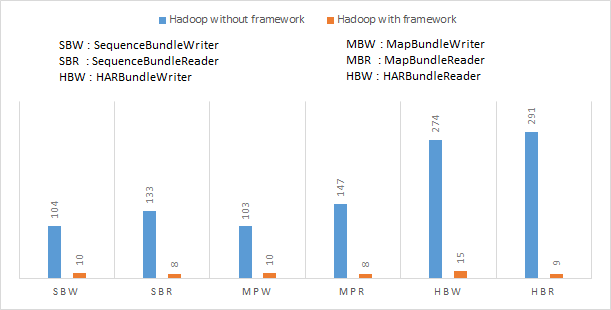
\includegraphics[width=0.45\textwidth]{files-chart}
	\caption{Comparing File Writers and readers without and with using framework }
	\label{fig:files-chart}
\end{figure}

\begin{lstlisting}[caption = Comparing File Writer instance in java and SequenceBundleWriter instance in Hadoop Image Processing framework ]

//Sample File Writing in Java

File file = new File("abc.txt");
FileWriter fw=new FileWriter(file);
fw.append(val)
fw.close();

//Sample BundleFile Writing in Hadoop using Framework

BundleFile file = new BundleFile("abc.seq");
SequenceBundleWriter sbw=new SequenceBundleWriter(file);
sbw.append(himage);
sbw.close();

\end{lstlisting}


\section{Conclusion}
This paper has decribed our framework fo image processing for large scale image processing applications on the MapReduce framework. The framework is designed to abstract the technical details of Hadoop's powerful MapReduce framework and provide a way for users who want to process large image datasets. We provided a how the images can be stored in different hadoop file format and efficient access within Map Reduce pipeline and simple modules to make the framework more easier. By providing interoperability between different image data types we give the user to process the images using different open-source image processing libraries. Finally, we provide a way to overcome the loss of image headers after processing which are most useful for image processing and vision applications.

With these features, the framework brings a new level of transparency and simplicity for creating large-scale image processing applications over Hadoop's MapReduce framework. The paper describes to example applications built using the framework to demonstrate the power of the framework. We hope that this level of abstractness to use Hadoop MapReduce framework will enhance the ability to create large-scale image processing applications with ease.

\section{Future Work}
In the near future we hope to extend the framework into a full-fledged multimedia processing framework. We would like to improve framework such that audio and video processing over hadoop is done with ease. We also intend to add a CUDA module for using the graphics card for processing the images. Finally, we intend to wrap our system into an highly parallelized open-source hadoop multimedia processing framework and perhaps provide a sample web-based graphic user interface with all image processing applications.  

	\bibliography{references}
	\bibliographystyle{IEEEtran}

\end{document}

